% Chapter Template

\chapter{Results - Rubiks' Cube} % Main chapter title

\label{Chapter5} % Change X to a consecutive number; for referencing this chapter elsewhere, use \ref{ChapterX}

%----------------------------------------------------------------------------------------
%	SECTION 1
%----------------------------------------------------------------------------------------

\section{2x2x2}

\subsection{Rubiks}

1000 seq 30 shuffles training each target network update seen 1.1\% of all puzzles
199 of the 200 perfectly shuffled got solved well under 1h (median 83 seconds), only one outlier took about 67 minutes.


\newgeometry{top=0mm, bottom=0mm, left=0mm, right=0mm}
\begin{landscape}
\centering\vspace*{\fill}
\begin{figure}[H]
\centering
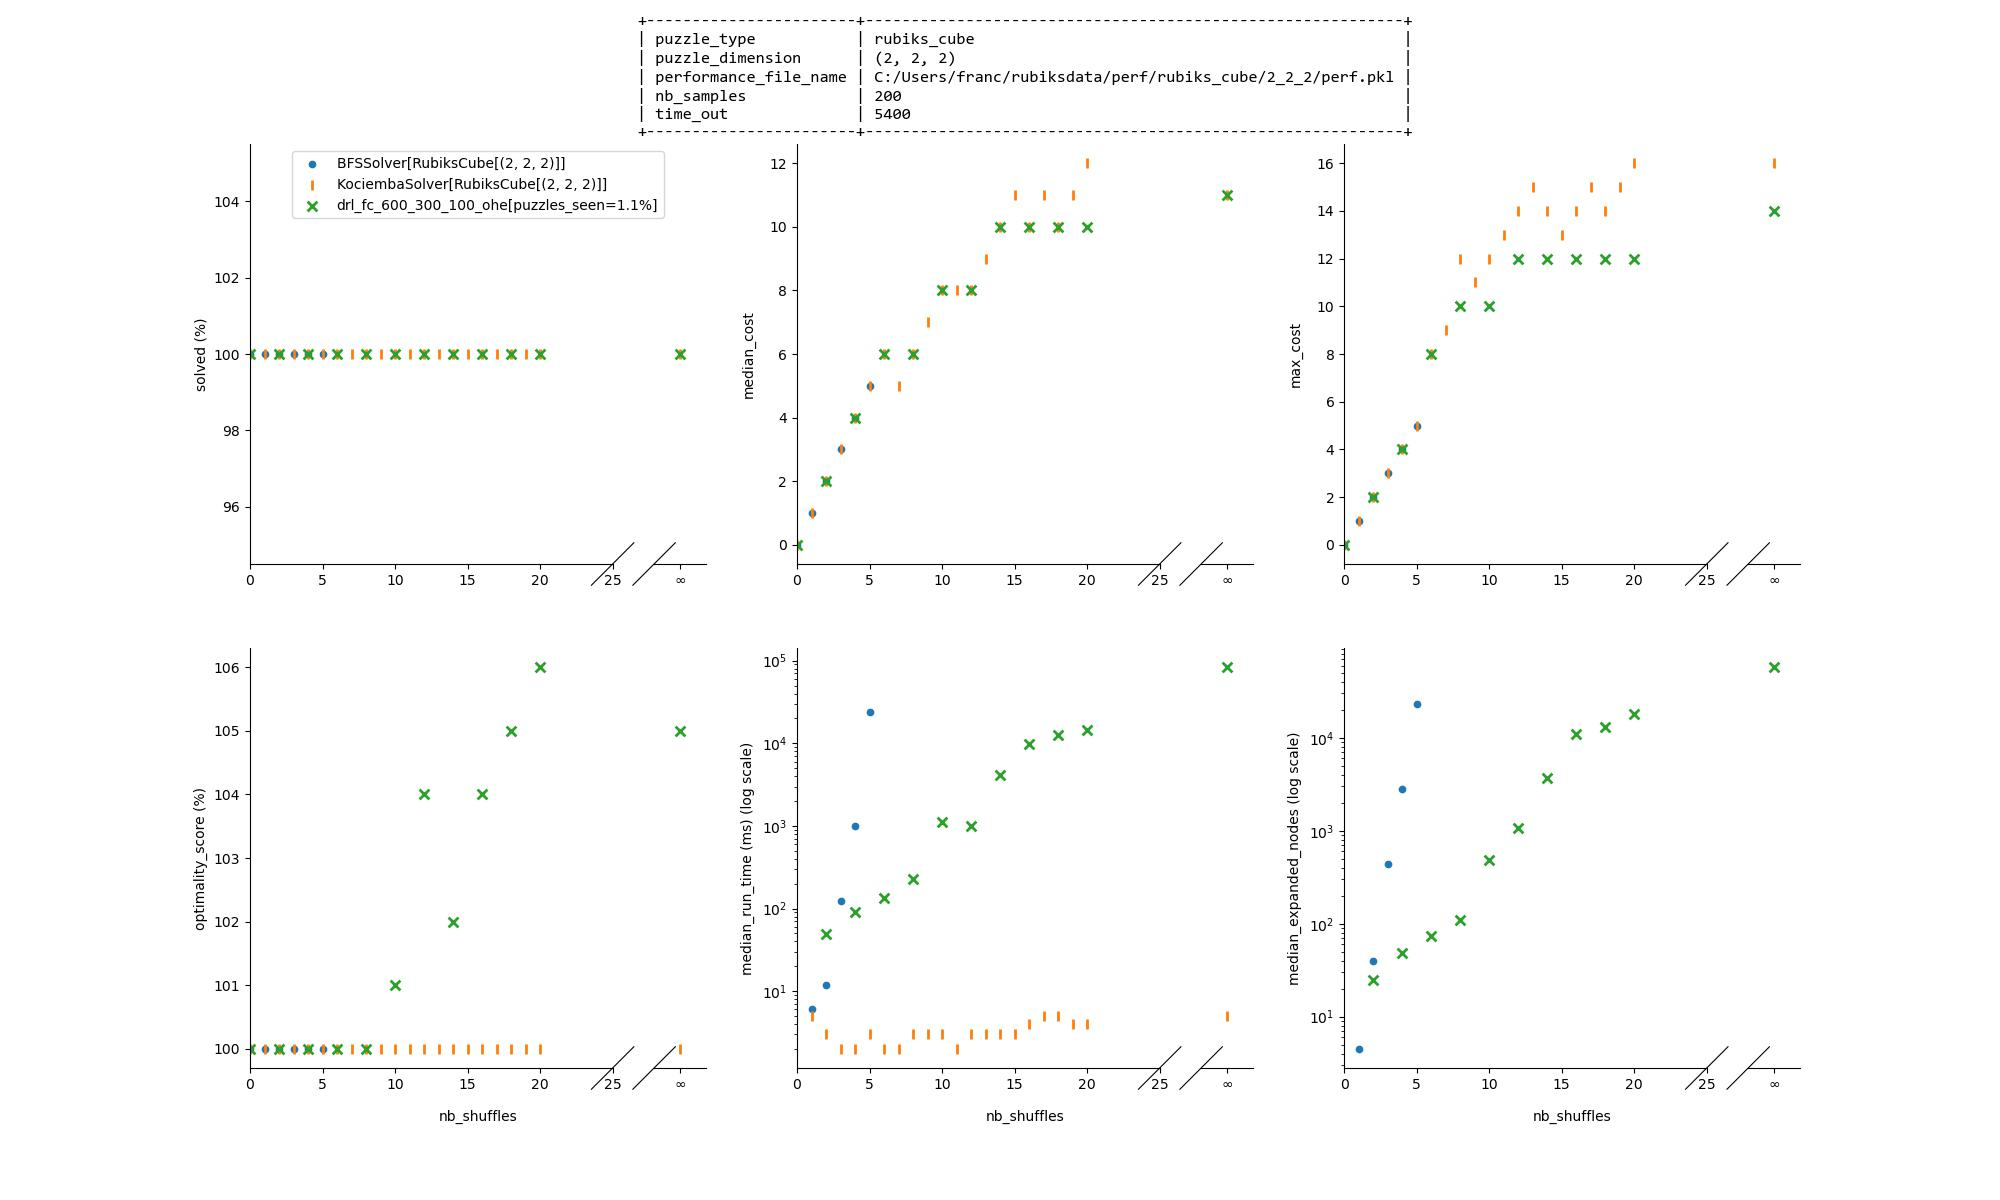
\includegraphics[scale=0.50]{./Figures/222RCPerformance.jpeg}
%\decoRule
\caption[222RCPerformance]{Solvers' performance comparison 2x2x2 RC}
\label{fig:222RCPerformance}
\end{figure}
\vfill
\end{landscape}
\restoregeometry


\subsection{Random goal}

not very successful with DRL. Seems to not even be doing better than BFS and basically impractical for nb\_shuffles $\geq$ 4.
\\
I will try with DL trained from Kociemba solutions, to see if $A^{*}$ with this DL heuristic finds more elegant solutions than Kociemba

\newgeometry{top=0mm, bottom=0mm, left=0mm, right=0mm}
\begin{landscape}
\centering\vspace*{\fill}
\begin{figure}[H]
\centering
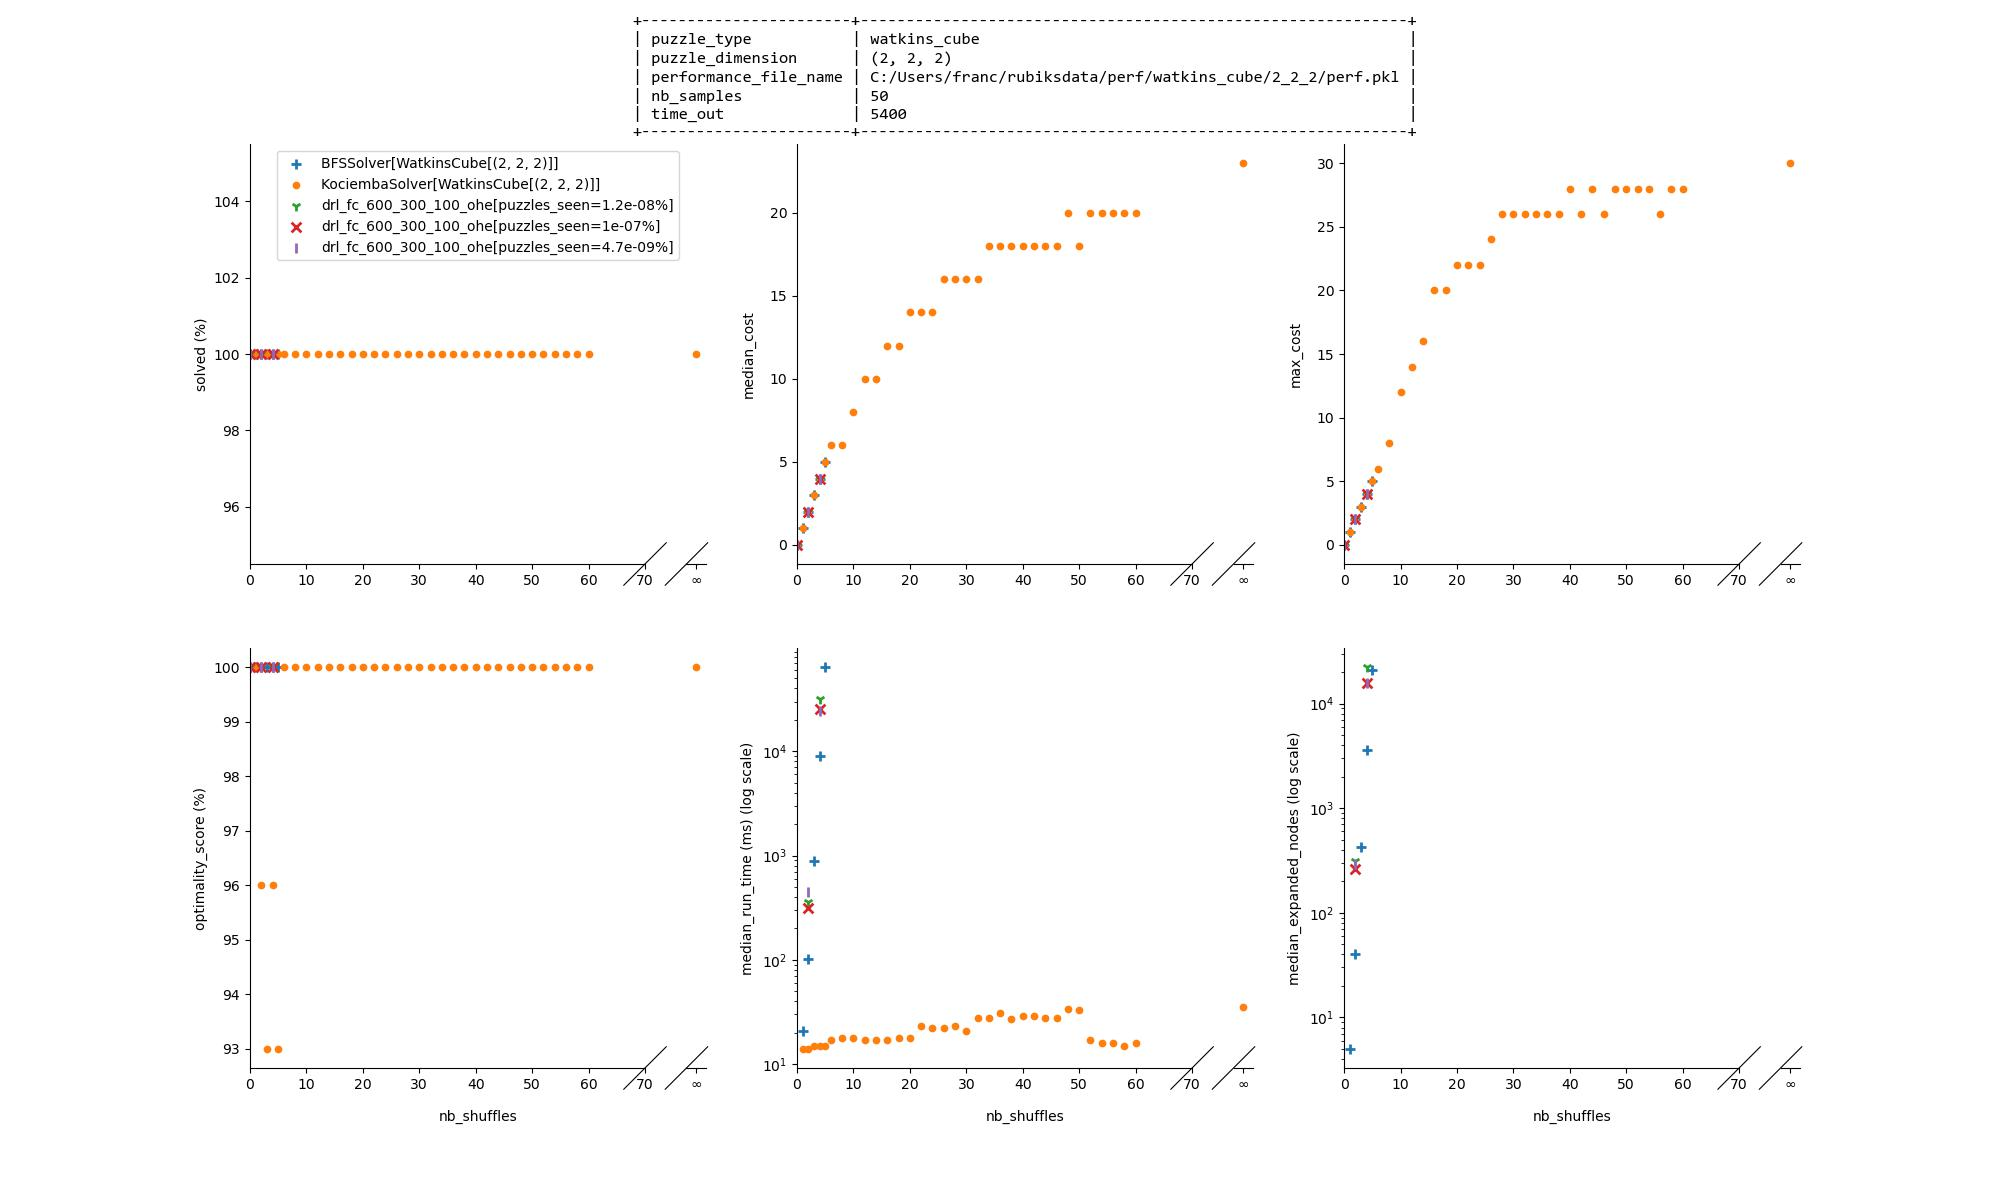
\includegraphics[scale=0.50]{./Figures/222WCPerformance.jpeg}
%\decoRule
\caption[222RCPerformance]{Solvers' performance comparison 2x2x2 Random-Goal-RUbik's}
\label{fig:222WCPerformance}
\end{figure}
\vfill
\end{landscape}
\restoregeometry

%-----------------------------------
%	SUBSECTION 1
%-----------------------------------
\section{3x3x3}

For now just showing Kociemba as a baseline. Will first try out DL trained on data generated from Kociemba, then will try out DRL. If unsuccessful or too slow, might try similar to paper using DQL/MC search.

\newgeometry{top=0mm, bottom=0mm, left=0mm, right=0mm}
\begin{landscape}
\centering\vspace*{\fill}
\begin{figure}[H]
\centering
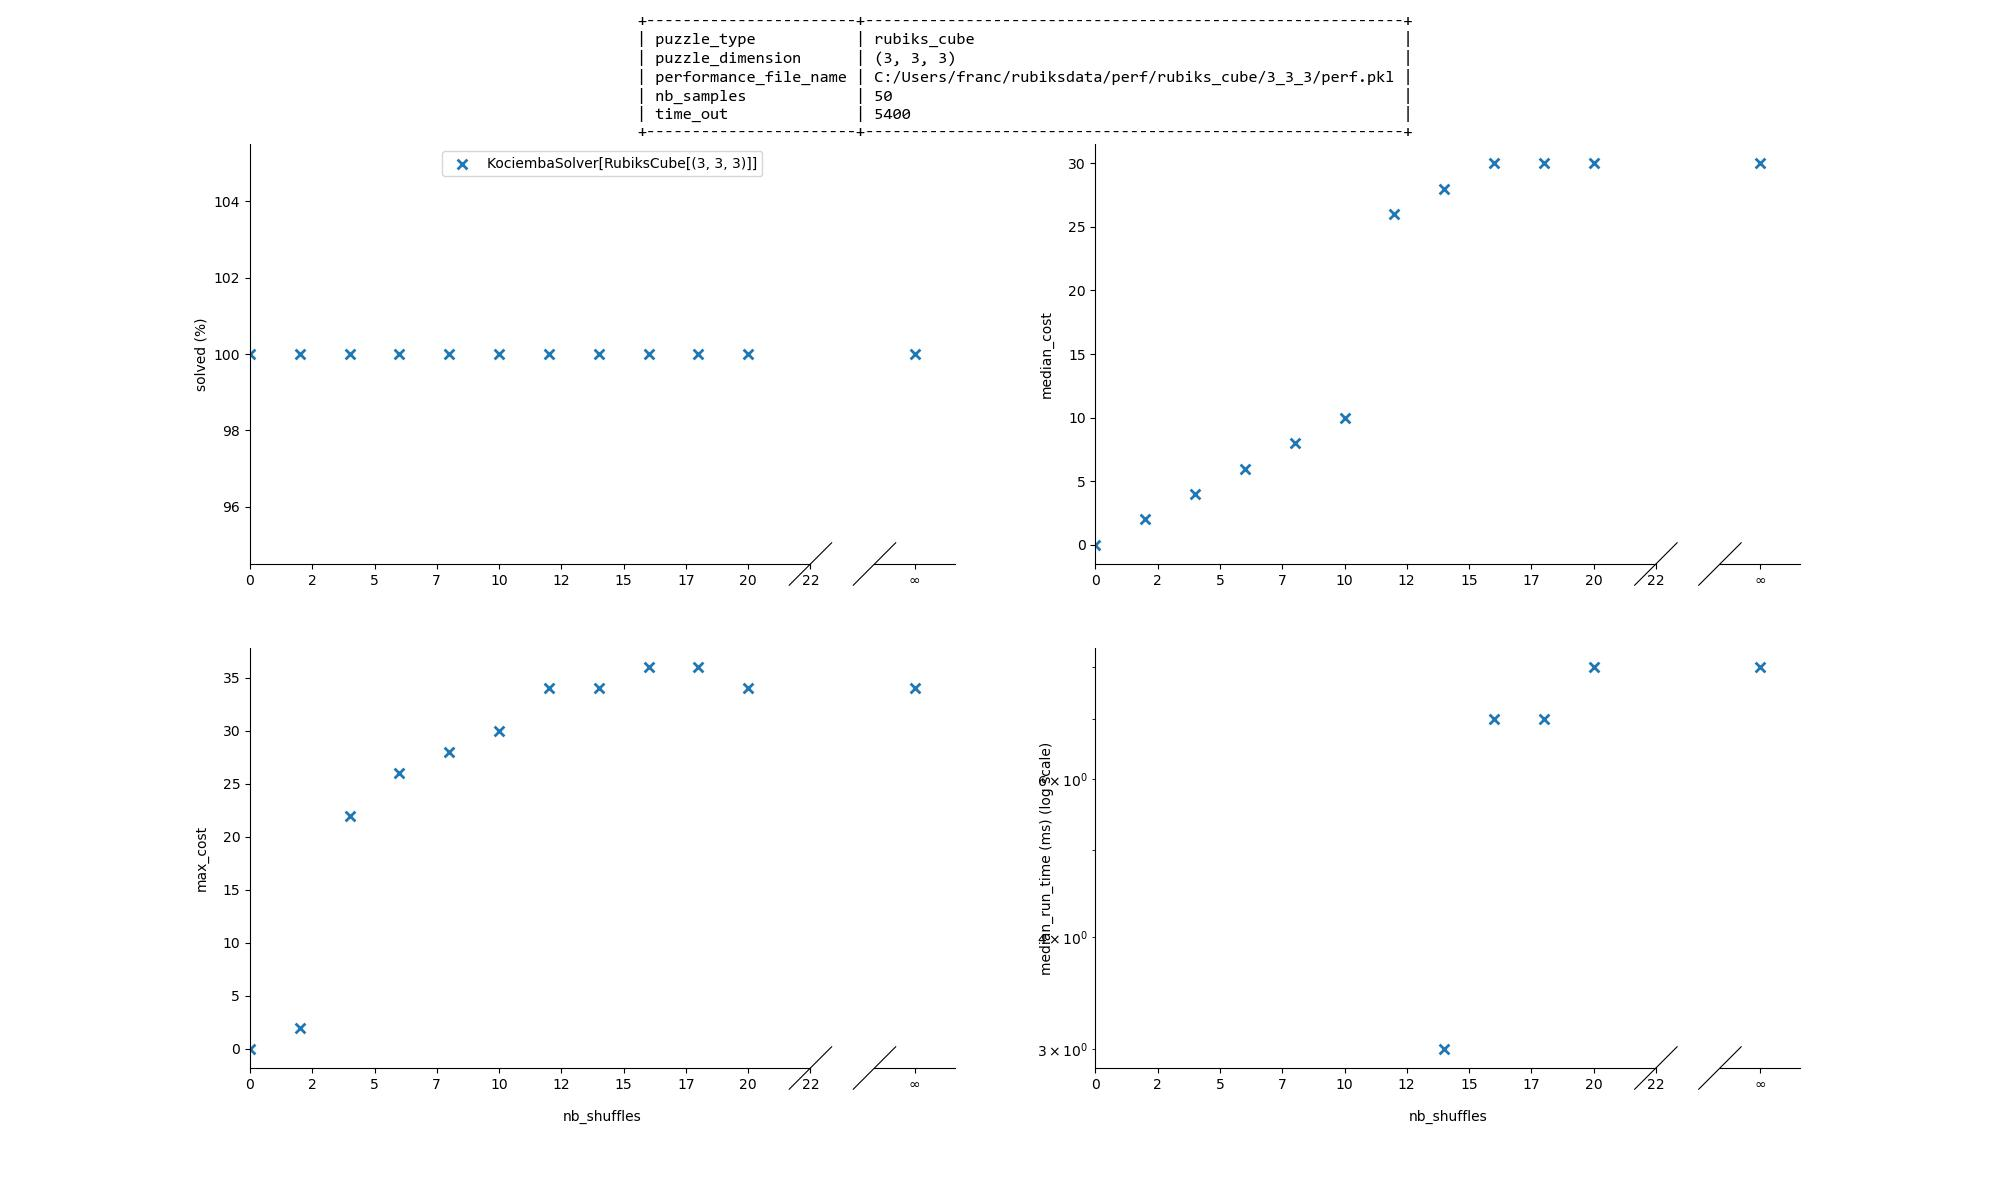
\includegraphics[scale=0.50]{./Figures/333RCPerformance.jpeg}
%\decoRule
\caption[333RCPerformance]{Solvers' performance comparison 3x3x3 RC}
\label{fig:333RCPerformance}
\end{figure}
\vfill
\end{landscape}
\restoregeometry

